\section{Tecnología \glsentryshort{xdp}}
\label{TecnologiaXDP}

La tecnología \gls{xdp}, es una tecnología para procesar paquetes, programable, de alto rendimiento e integrada en el \textit{datapath} del Kernel de Linux. Esta tecnología se basa en ejecutar \textit{bytecodes} \gls{bpf} cuando la interfaz sobre la cual está anclado un programa \gls{xdp} recibe un paquete. Esto habilita que ciertas decisiones para según que paquetes, se realicen lo antes posible casi en la propia interfaz, quitándose de encima todas las capas del \textit{stack} que harían operaciones redundantes.\\
\par

Pero el hecho de que se ejecute casi en la propia interfaz no es la única razón del alto rendimiento de los programas \gls{xdp}. Otras decisiones que han sido vitales para hacer de esta tecnología una pieza clave para las nueva generación de herramientas\footnote{\url{https://git.kernel.org/pub/scm/linux/kernel/git/netdev/net-next.git}} en Linux.

\begin{itemize}
    \item No se reserva memoria mientras se hace el procesamiento de paquetes con \gls{xdp}.
    \item No se emplea las estructuras \texttt{sk\_buff} para gestionar la información de metadatos de los paquetes, en cambio se hace uso de una estructura \texttt{xdp\_buff} la cual no contiene tanta información en exceso. 
    \item No se permiten bucles, ni un número excesivo de iteraciones en los programas anclados a la \gls{nic}.
    
\end{itemize}


\par

El funcionamiento de un programa \gls{xdp} se basa generalmente en analizar un paquete, editarlo en caso de que sea necesario y por último, devolver un código de retorno que indique que se debe hacer con dicho paquete. Los códigos de retorno \gls{xdp}, se utilizan para determinar qué acción se va a tomar con el paquete, estas acciones pueden ser muy variadas, desde hacer que el paquete sea descartado, hasta delegarlo al \textit{stack} de red para que se encargue este del procesado, o reenviar el paquete para que sea transmitido de nuevo. \\
\par

Antes se mencionaba que los programas \gls{xdp}, consistían en ejecutar \textit{bytecodes} \gls{bpf} cuando llega un paquete a la interfaz donde está cargado el programa, pero, ¿Qué relación existe entre \gls{xdp} y \gls{bpf}? Resulta que todos los programas \gls{xdp} que se escriben en un C restringido, se compilarán haciendo uso del compilador de \textbf{clang}\footnote{Compilador de tipo frontend de referencia de la familia del lenguaje C.} como \textit{frontend} y del compilador \textbf{LLVM}\footnote{Infraestructura para implementar compiladores de forma agnóstica al lenguaje a compilar, generalmente usado como compilador de Backend.} como \textit{backend}, para conseguir un \textit{bytecode} \gls{bpf}.\\
\par

La motivación de esta ``traducción" radica en  que los programas XDP son cargados en el Kernel a través de la llamada al sistema \gls{bpf}, indicando que se trata de un tipo de programa \gls{xdp} con la macro, \texttt{BPF\_PROG\_TYPE\_XDP}. De esta forma, se permite reutilizar los mecanismos de carga de \textit{bytecodes} en el Kernel utilizados con \gls{bpf}, pero en este caso con \gls{xdp} estarán únicamente enfocados en la carga de dichos \textit{bytecodes} en la \gls{nic}. Por lo que, \gls{xdp} se podría ver como un \textit{framework} \gls{bpf} diseñado para trabajar en la interfaz, con limitaciones y pautas de desarrollo muy marcadas para conseguir que la tecnología sea de alto rendimiento \cite{xdp1}.\\
\newpage

\subsection{Modos de operación}

\begin{table}[h!]
\centering
\resizebox{\textwidth}{!}{%
\begin{tabular}{|l|l|}
\hline
\rowcolor[HTML]{EFEFEF} 
\multicolumn{1}{|c|}{\cellcolor[HTML]{EFEFEF}{\color[HTML]{24292E} \textbf{Modo de Operación}}} & \multicolumn{1}{c|}{\cellcolor[HTML]{EFEFEF}{\color[HTML]{24292E} \textbf{Descripción}}}                                                                                                                                                                                                                                                                           \\ \hline
\texttt{OFFLOADED XDP}                                                                                   & \begin{tabular}[c]{@{}l@{}}En este modo de operación, el programa XDP se carga directamente en la propia NIC \\  en lugar de ser ejecutado en la CPU del host. Al sacar la ejecución fuera del sistema y\\  delegarla a la propia NIC, este modo tiene las mejores ganancias de rendimiento.\end{tabular}                                                          \\ \hline
\texttt{NATIVE XDP}                                                                                      & \begin{tabular}[c]{@{}l@{}}En este modo de operación los programas XDP se ejecutan lo antes posible una vez\\ recibidos por el driver de la NIC. Este modo no está disponible en todos los drivers\\ ( Todos aquellos que permiten este modo gestionan la macro XDP\_SETUP\_PROG ).\end{tabular}                                                                   \\ \hline
\texttt{GENERIC XDP}                                                                                     & \begin{tabular}[c]{@{}l@{}}Este modo de operación se proporciona como un modo de prueba para desarrollar \\ programas XDP. Está soportado desde la versión 4.12 del Kernel y se puede utilizar\\ este modo por ejemplo en pares de Veths.\\  \\ Nótese que no se obtendrá el mismo rendimiento que con los dos modos anteriores\\ de funcionamiento.\end{tabular} \\ \hline
\end{tabular}
}
\caption{Resumen modos de operación en XDP}
\label{tab:xdpOPmodes}
\end{table}


\subsection{Procesamiento de paquetes}

Una vez que se ha analizado el paquete, se ha filtrado por los valores de sus cabeceras o se ha modificado, se tendrá ya pensada una acción a realizar con este paquete. Para expresar dicha acción, se hará uso de los códigos de retorno \gls{xdp} \cite{xdp2}.
\begin{itemize}
    \item  \texttt{XDP\_DROP}, se descarta el paquete, esto se hará lo antes posible en la etapa de recepción de los paquetes. Siendo un mecanismo de muy útil para proteger al sistema de ataques \gls{dos}, ya que cada paquete implicará una cantidad ínfima de procesamiento.
    \item  \texttt{XDP\_ABORTED}, este código de retorno se utilizará para denotar un error, ya que descartará el paquete y además generará una excepción del tipo \texttt{xdp\_exception}.
    \item  \texttt{XDP\_PASS}, con este código de retorno se delegarán los paquetes al \textit{stack} de red.
    \item  \texttt{XDP\_TX}, este código de retorno \gls{xdp}, se utiliza para reenviar el paquete a la misma interfaz por la cual se recibió para su transmisión.
    \item  \texttt{XDP\_REDIRECT}, este código de retorno generalmente su emplea cuando se hace un reenvío del paquete desde una \gls{nic} a otra \gls{nic}.
\end{itemize}

Todos los códigos de retorno se pueden encontrar definidos como una enumeración en el archivo de cabecera llamado \texttt{<linux/bpf.h>}. En el bloque \ref{code:xdp_codes} se puede ver dicha definición.

\begin{lstlisting}[language=C, style=C-color, caption={Definición de códigos de retorno XDP},label=code:xdp_codes]
    enum xdp_action {
        XDP_ABORTED = 0,
        XDP_DROP,
        XDP_PASS,
        XDP_TX,
        XDP_REDIRECT,
    };
\end{lstlisting}
\vspace{0.2cm}


\begin{figure}[ht]
    \centering
    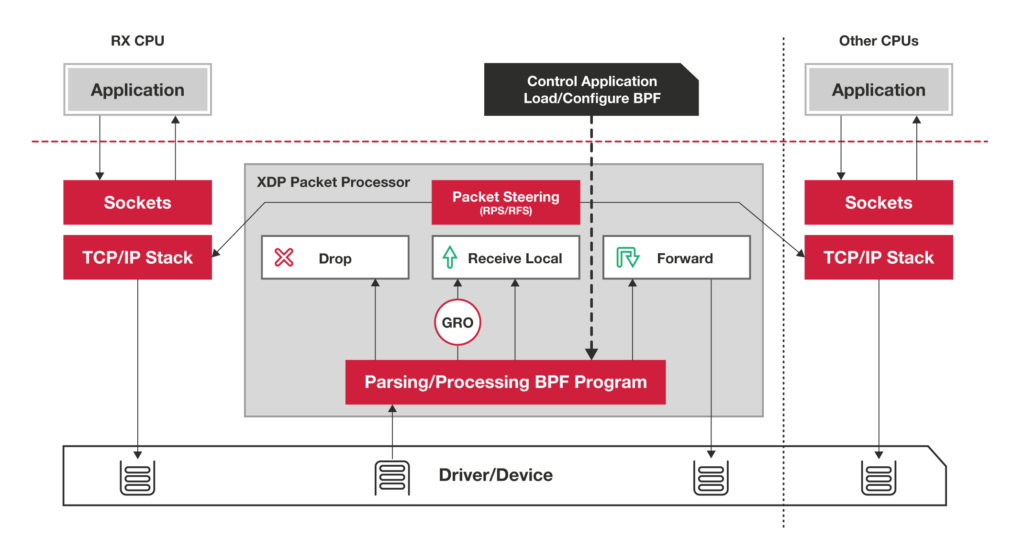
\includegraphics[width=14.5cm]{archivos/img/teoria/xdp-packet-processing.png}
    \caption{Procesamiento de paquetes con XDP}
    \label{fig:xdp_codes}
\end{figure}

\subsection{Limitaciones con \glsentryshort{xdp}}

En esta subsección se indicarán todas las limitaciones que se pueden encontrar a la hora de trabajar con la tecnología \gls{xdp}, además de ciertos detalles que hayan parecido limitaciones aunque sean características de la propia tecnología en favor de ofrecer más seguridad.

\subsubsection{Accesos a memoria y comprobación de limites}

El acceso a los paquetes se hará de modo directo a la memoria, sabiendo que el verificador se asegurará de que dichos accesos sean seguros. Sin embargo, hacer esto en tiempo de ejecución para cada acceso a memoria resultaría en una sobrecarga de rendimiento significativa. Por lo tanto, lo que el verificador hace es comprobar que el programa \gls{xdp} hace su propia comprobación de límites, en su propia lógica \cite{xdp1}. Por ejemplo, si con un programa se están parseando cabeceras Ethernet se haría la comprobación de limites indicada en el bloque \ref{code:xdp_lim}.
%code 
\begin{lstlisting}[language=C, style=C-color, caption={Comprobación de limites en XDP},label=code:xdp_lim]
 SEC("xdp_prog")
 int xdp_ether_parser(struct xdp_md *ctx){
 
	 void *data_end = (void *)(long)ctx->data_end;
	 void *data = (void *)(long)ctx->data;
     int hdrsize = sizeof(struct ethhdr);
    
     /*  Comprobación de limites */
     if (data + hdrsize > data_end)
		 return -1;
		
	 return XDP_PASS;
 }
\end{lstlisting}
\vspace{0.2cm}

En el caso de que se manejen más tipos de cabeceras posteriormente, habría que hacer también comprobaciones de límites con los distintos tipos de cabeceras. De forma general, las definiciones de los parsers se suelen definir aparte como funciones \textit{inline} y  se llaman desde el propio programa \gls{xdp} para hacer el código más legible. \\
\par

Cuando el verificador realiza su análisis estático en tiempo de carga, rastreará todas las direcciones de memoria utilizadas por el programa, y buscará comparaciones con el puntero data-end, el cual será puesto al final del paquete en tiempo de ejecución. En el momento que el verificador crea que puede darse un acceso indebido, descartará el programa \gls{xdp}.


\subsubsection{Bucles y funciones inline}

Puesto que XDP se puede ver como un \textit{framework} \gls{bpf}, también comparte sus limitaciones como son las limitaciones de llamadas a funciones y los bucles. Por ello, muchas de las funciones que se van a desarrollar en los programas \gls{xdp} necesitarán ser de un carácter \textit{inline} ( \texttt{\_\_always\_inline}) para que así el compilador las sustituya tal cual en código.\\
\par
De esta forma se consigue una mejora de rendimiento, ya que no hay que hacer una llamada a una función con todo lo que ello conlleva (Cambio de contexto, salvado de registros, incremento del PC), y se consigue evitar las limitaciones de llamadas a funciones del verificador \cite{xdp2}.\\
\par

En cuanto a la limitación de los bucles, \gls{bpf} no soporta los bucles, por lo que se deberá desenrollar los bucles. Pero, ¿Qué significa desenrollar un bucle? Atendiendo al bloque \ref{code:xdp_loops} podemos hacernos una idea. 

%code 
\begin{lstlisting}[language=C, style=C-color, caption={Loops Unrolling},label=code:xdp_loops]

    #pragma unroll
    for ( int j = 0; j < 4 ; j++)
     printf("Contador %d \n", j);
    
    
    // Si lo desenrollamos, quedaría así:
    printf("Contador %d \n", 0);
    printf("Contador %d \n", 1);
    printf("Contador %d \n", 2);
    printf("Contador %d \n", 3);

\end{lstlisting}
\vspace{0.5cm}

Para conseguir esto debemos añadir la siguiente declaración antes del bucle \textit{pragma unroll}. Esta declaración solo es válida cuando el numero de iteraciones del bucle es conocida en tiempo de compilación y no supera el numero máximo de instrucciones que admite el verificador del Kernel (4096) \cite{xdp1}.